\section{Test interoperabilità con C/C++}


In questo test empirico viene utilizzata la libreria Benchee
che ci permette di valutare le performance di esecuzione di
funzioni, in particolare le funzioni da eseguire saranno due funzioni
scritte in Elixir, ed altre due con il meccanismo di integrazione
di cui si è parlato nel paragrafo \ref{subsec:mysubsection}
Il problema che si vuole risolvere è il problema definito
nell'equazione \ref{eq:problem_interoperability}.
\begin{equation}
	[n_{1},n{_2}...n{_m}] \rightarrow [\sum_{i=1}^{n_{1}}i,\sum_{i=1}^{n_{2}}i,...,\sum_{i=1}^{n_{m}}i]
  \rightarrow [sum_{1},sum_{2},...,sum_{m}]
  \label{eq:problem_interoperability}
\end{equation}

Le funzioni implementate prendono come input una lista
di interi, e si vuole restituire una lista che contiene
i risultati dell'equazione \ref{eq:problem_interoperability}.

L'input di riferimento è: [ 1000000, 2000000, 5000000], non si
sono scelti numeri troppo piccoli per avere un gap visibile
tra le strategia di implementazione adottate.

Le funzioni si occupano di calcolare il risultato della somma
\ref{eq:problem_interoperability} per ogni elemento e
restituirà una lista con il relativo risultato per ogni elemento.

Le funzioni sono implementate con 4 strategie differenti:
\begin{enumerate}
	\item list\_sum\_recursive(): Funzione implementata in elixir
	tramite ricorsione.
	\item list\_sum\_recursive\_tail(): Funzione implementata in elixir
	tramite ricorsione ottimizzata, dove l'ultima istruzione è la
	chiamata ricorsiva, in modo che elixir ottimizza la ricorsione
	con la tail optimization.
	\item list\_sum\_port(): Funzione implementata in C++, Elixir interagisce
	con il codice tramite il meccanismo IPC Port.
	\item list\_sum\_iterative\_nif(): Funzione implementata in C++, Elixir
	interagisce con il codice C++ tramite il meccanismo NIF.
\end{enumerate}

Tutte le funzioni elixir che seguiranno in questo paragrafo
vengono messe dentro il modulo SpeedSum
come nel Listing \ref{lst:speedSum}:

\begin{lstlisting}[language=elixir,captionpos=b,
	caption={Modulo di riferimento},
	label={lst:speedSum}]
defmodule Speedsum do
....
# Funzioni implementate
....
end


\end{lstlisting}

% --------------------------------------------

\subsection{Funzione ricorsiva}
Nel Listing \ref{lst:listsumrecursive} è riportata l'implementazione
della funzione ricorsiva che risolve il problema definito sopra.

\begin{lstlisting}[language=elixir,captionpos=b,
	caption={Funzione list\_sum\_recursive()},
	label={lst:listsumrecursive}]
def list_sum_recursive(list) when is_list(list) do
  Enum.map(list, fn x -> sum_recursive(x) end)
end

#caso base
defp sum_recursive(0), do: 0

defp sum_recursive(n), do: n + sum_recursive(n - 1)
\end{lstlisting}

%---------------------------------------------------------------------
\subsection{Funzione ricorsiva ottimizzata}
Nel Listing \ref{lst:listsumrecursivetail} è riportata l'implementazione
della funzione ricorsiva ottimizzata con il metodo tail optimization,
Elixir come vedremo dai risultati del Benchmark risolve il problema
definito in modo molto più veloce, come si può vedere dal codice
implementato, per far sì che il passo ricorsivo sia l'ultima
istruzione della funzione, necessita di passare lo stato della
somma come parametro della funzione.

\begin{lstlisting}[language=elixir,captionpos=b,
	caption={Funzione list\_sum\_recursive\_tail()},
	label={lst:listsumrecursivetail}]
# Funzione di somma ricorsiva ottimizzata
def list_sum_recursive_tail(list) when is_list(list) do
  Enum.map(list, fn x -> sum_recursive_tail(x, 0) end)
end
  
#caso base
defp sum_recursive_tail(0, acc), do: acc

defp sum_recursive_tail(n, acc) when n > 0 do
  sum_recursive_tail(n - 1, acc + n)
end
\end{lstlisting}

%---------------------------------------------------------------------

\subsection{Funzione implementata in C++ tramite Port}

Con l'Inter process communication in Erlang ed Elixir, si può comunicare
con un processo esterno tramite il meccanismo Port, e si può comunicare con
i cosiddetti file descriptor, nel nostro caso è stata implementata la
comunicazione usando lo standard input e lo standard output. 
Per la comunicazione si deve scegliere un formato di codifica e decodifica, per non complicare le cose si è scelto
si è scelta una comunicazione line by line, dove la lista viene inviata
da Elixir nel formato "$n_{1},n_{2},...,n_{m}$" scegliendo come
carattere delimitatore la ",".

Il codice C++ che risolve il nostro problema è riportato nel Listings
\ref{lst:list_sum_port}

\begin{lstlisting}[language=cpp,captionpos=b,
	caption={Funzione list\_sum\_port()},
	label={lst:list_sum_port}]
#include <algorithm>
#include <iostream>
#include <sstream>
#include <string>
#include <vector>
	
//Funzione che prende in input una stringa
//di interi separati da un delimitatore e
//restituisce un vector di interi
std::vector<long int> tokenizeToIntVector(const std::string &str,
                                          char delimiter) {
  std::vector<long int> tokens;
  std::stringstream ss(str);
  std::string token;
  while (std::getline(ss, token, delimiter)) {
    tokens.push_back(
      std::stol(token));
	}
	return tokens;
}
	
int main() {
  std::string line;
  // Ascolta lo standard input line by line
  while (std::getline(std::cin, line)) {

    char delimiter = ',';

    std::vector<long> numbers = tokenizeToIntVector(line, delimiter);
    std::vector<long> results;

    for (auto &n : numbers) {
      long sum = 0;
      for (int i = 0; i <= n; i++) {
        sum += i;
      }
      results.push_back(sum);
    }

    // Stampa sullo standard output una stringa
    // nello stesso formato di ricezione
    for (int i = 0; i < results.size() - 1; i++) {
      std::cout << results[i] << ",";
    }
    std::cout << results[results.size() - 1] << std::endl;
  }
  return 0;
}

\end{lstlisting}

Si può compilare il programma C++ tramite il compilatore gcc:
\begin{lstlisting}[language=none]
g++ -o list_sum_port <source-directory>/list_sum_port.cpp
\end{lstlisting}

Nel Listing \ref{lst:listsumportelixir} è riportata la funzione
che comunica con il programma C++ scritto per la risoluzione
del problema definito.

\begin{lstlisting}[language=elixir,captionpos=b,
	caption={Funzione list\_sum\_port()},
	label={lst:listsumportelixir}]

def list_sum_port(list) when is_list(list) do

  # Apertura del Port
  port = Port.open({:spawn_executable, "./priv/list_sum_port"},
                   [:binary,:use_stdio])

  # encoding del messaggio da inviare al port
  message = Enum.join(list,", ")

  # invio del messaggio al port
  Port.command(port, "#{message}\n")

  receive do
    {^port, {:data, result}} ->
      String.trim(result)

    {^port, {:exit_status, status}} ->
      IO.puts("Processo port terminato con codice di uscita #{status}")
  after
    1000 ->
      IO.puts("Timeout")
  end
  Port.close(port)
end
\end{lstlisting}

%-------------------- Funzione NIF -----------------------
\subsection{Funzione implementata in C++ tramite NIF}

Nel caso del metodo NIF non c'è bisogno di decidere un
metodo di codifica e decodifica, ma bisogna affidarsi
all'interfaccia che Erlang ci mette a disposizione per
far interfacciare il codice C con Elixir, l'interfaccia
supporta solo il C, quindi per poter utilizzare codice C++
si devono fare le dovute conversioni.
Nel Listing \ref{lst:list_sum_nif} è riportato il codice
NIF per la risoluzione del problema definito.


%// gcc -fPIC -shared -o elixir_nif.so elixir_nif.c -I $ERL_ROOT/usr/include/
\begin{lstlisting}[language=cpp,captionpos=b,
	caption={Funzione NIF},
	label={lst:list_sum_nif}]
#include "erl_nif.h" 
#include "string.h"
#include <vector>
	
	
// funzione per riempire un vector da una lista di Elixir
inline bool fillVector(ErlNifEnv* env,
                      ERL_NIF_TERM listTerm,
                      std::vector<long int>& result) 
{
  unsigned int length = 0;
  if (!enif_get_list_length(env, listTerm, &length)) {
    return false;
  }
	
  long int actualHead; 
  ERL_NIF_TERM head;
  ERL_NIF_TERM tail;
  ERL_NIF_TERM currentList = listTerm;
	
  // O(n), scorre tutta la lista
  for (unsigned int i = 0; i < length; ++i) {
    if (!enif_get_list_cell(env, currentList, &head, &tail)) {
      return false;
    }
    currentList = tail;
    if (!enif_get_long(env, head, &actualHead)) {
      return false;
    }
    result.push_back(actualHead);
  }
  return true;
  }
	
static ERL_NIF_TERM list_sum_iterative_nif(ErlNifEnv* env,
                                          int argc,
                                          const ERL_NIF_TERM argv[]) {
	
  std::vector<long int> a;
	
  if (!fillVector(env, argv[0], a)) {
    return enif_make_badarg(env);
  }
	
  //creazione dell'array per i risultati da restituire
  ERL_NIF_TERM results[a.size()];
	
  for(int i=0; i < a.size() ;++i){
    long int  sum = 0;
    for (int j = 1; j <= a[i]; j++) {
    sum += j;
  }

  ERL_NIF_TERM  temp = enif_make_long(env, sum);
  results[i] = temp;
  }

  ERL_NIF_TERM list = enif_make_list_from_array(env, results , a.size());
	
  return list;
}
	
// Definizione delle funzioni NIF
static ErlNifFunc nif_funcs[] = {
  {"list_sum_iterative_nif", 1, list_sum_iterative_nif}
};

ERL_NIF_INIT(Elixir.SpeedSum, nif_funcs, NULL, NULL, NULL, NULL)
	
\end{lstlisting}

Come si può vedere il NIF implementato è composto da una funzione
ausiliaria che rserve per riempire il vettore dalla lista di Elixir,
dall'implementazione della funzione NIF list\_sum\_iterative\_nif(),
e dalla macro ERL\_NIF\_INIT.

Si può notare che tutti i tipi che devono essere letti
dalla VM devono essere degli ERL\_NIF\_TERM, che possono essere
letti e scritti utilizzando l'API messa a disposizione dall'installazione
di Erlang, che si trova nel file "erl\_nif.h".

Per utilizzare la funzione implementata, il codice deve essere compilato
come una libreria condivisa, con il compilatore gcc si può compilare
nel seguente modo:

\begin{lstlisting}[language=none]
g++ -fPIC -shared -o list_sum_iterative_nif.so \\
    list_sum_iterartive_nif.cpp -I $ERL_ROOT/usr/include/
\end{lstlisting}

La directory \$ERL\_ROOT dipende dall'installazione di Erlang,
per saperne il valore si può eseguire:
\begin{lstlisting}[language=none]
elixir -e "IO.puts :code.root_dir()"
\end{lstlisting}

Per eseguire la funzione esterna implementata, basta definire
nel modulo di riferimento il seguente codice:

\begin{lstlisting}[language=elixir,captionpos=b,
	caption={Funzione list\_sum\_port()},
	label={lst:listsumportelixir}]

def load_nif do
  :ok = :erlang.load_nif(
	    String.to_charlist("priv/list_sum_iterative_nif"),
		0)
end

def list_sum_iterative_nif(_n) do
  :erlang.nif_error("Errore nel caricamento nif")
end
\end{lstlisting}



%--------------------- ESECUZIONE ------------------------
\subsection{Esecuzione Test}

Per l'esecuzione del test come precedentemente detto
ci si è affidati alla libreria Benchee \cite{bencheeo54:online}.

Per includere la libreria Benchee, basta inserire nella funzione
deps del file \textbf{mix.exs} del progetto Elixir il nome
della libreria con la versione, la funzione diventa
quella del Listing \ref{lst:benchee_dependencies}.


\begin{lstlisting}[language=elixir,captionpos=b,
	caption={Dipendenze di Benchee},
	label={lst:benchee_dependencies}]
defp deps do
  [
  {:benchee, "~> 1.0", only: :dev},     
  {:benchee_html, "~> 1.0", only: :dev},
  ]
end
\end{lstlisting}

Viene inserito anche il plug-in della libreria
per visualizzare il report in formato html per
una visione più chiara del risultato.

Con la libreria Benchee sono state testate tutte e quattro le
strategie di implementazione usate, ed è stato aggiunta la strategia
di formattazione HTML per visualizzare i report, nel Listing \ref{lst:speedtest_function}.
 

\begin{lstlisting}[language=elixir,captionpos=b,
	caption={Funzione speed\_test()},
	label={lst:speedtest_function}]
def speed_test() do
  list_input = [1_000_000, 2_000_000,5_000_000]
  Benchee.run(
  %{
   "sum_recursive" => fn -> list_sum_recursive(list_input) end,
   "sum_recursive_tail" => fn -> list_sum_recursive_tail(list_input) end,
   "sum_iterative_nif" => fn -> list_sum_iterative_nif(list_input) end,
   "list_sum_port" => fn -> list_sum_port(list_input) end
   },
   warmup: 4,
   memory_time: 4,
   formatters: [
     Benchee.Formatters.HTML,
     Benchee.Formatters.Console
  ])
end
\end{lstlisting}

La funzione costruisce un report in HTML che riporta la Tabella
in figura \ref{fig:report_tab_interoperabilita}

\begin{figure}[!htp]
    \centering
    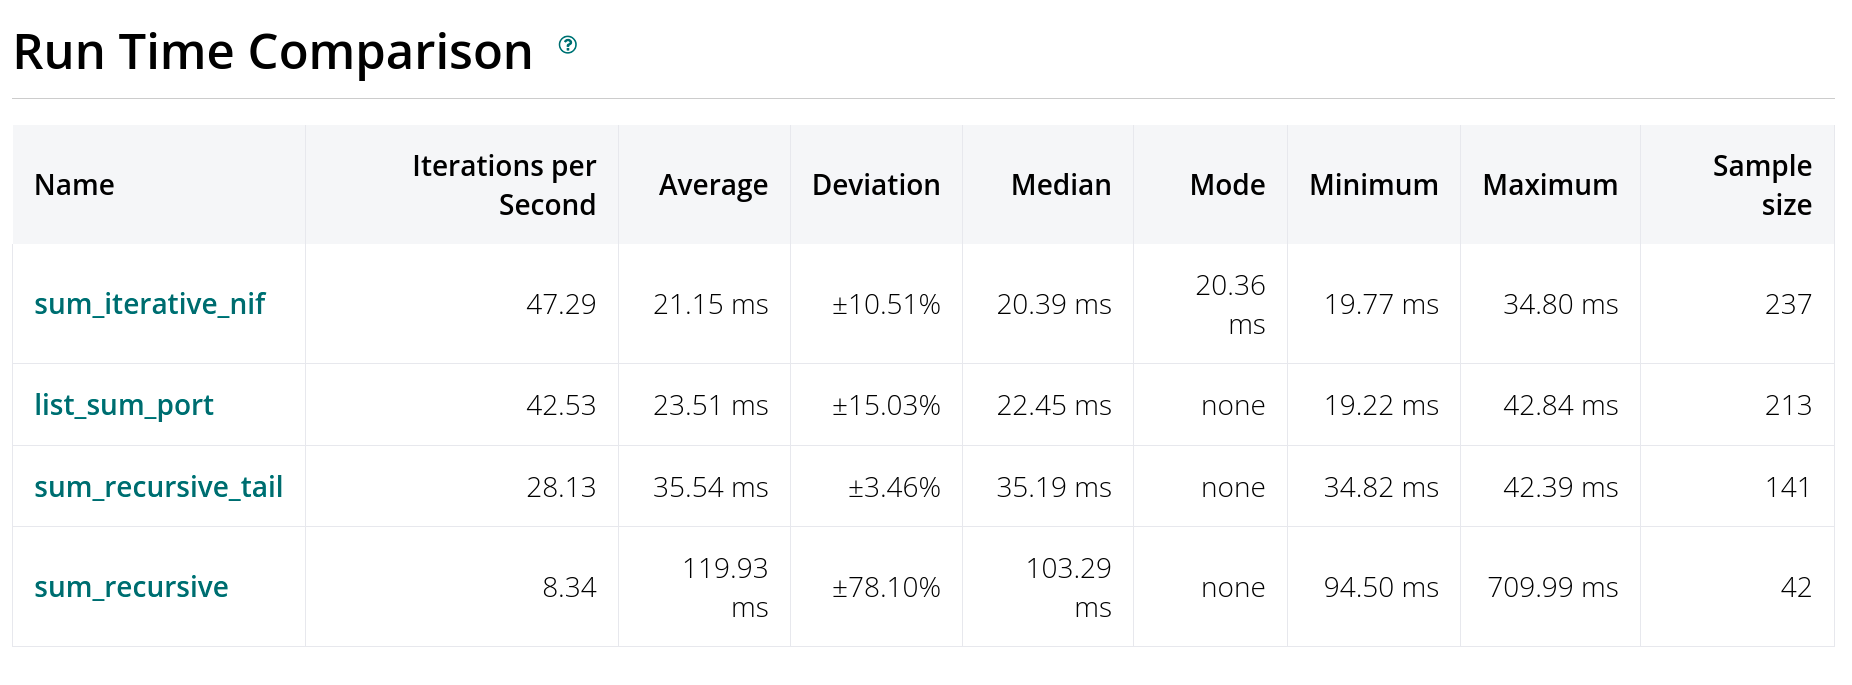
\includegraphics[keepaspectratio=true,scale=0.21]{images/tab_report.png}
	\caption{Report di Benchee}
  	\label{fig:report_tab_interoperabilita}
\end{figure}

\begin{figure}[!htp]
    \centering
    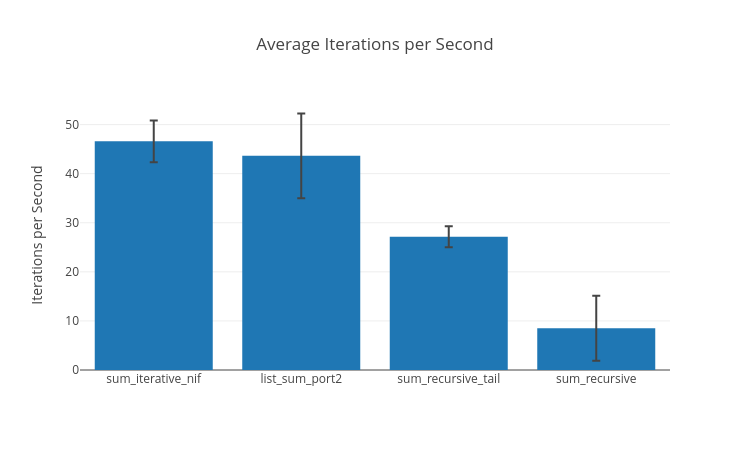
\includegraphics[keepaspectratio=true,scale=0.5]{images/newplot.png}
	\caption{Report a barre, iterazioni a secondo}
  	\label{fig:report_barre}
\end{figure}


Come possiamo notare le funzioni scritte in C++ risultano più veloci,
non ci sono grosse differenze tra il metodo NIF e il metodo con le Port,
per molti casi la strategia con le Port dovrebbe risultare la più conveniente.

Un fatto molto curioso sono le funzioni implementate in Elixir,
notiamo che la ricorsione ottimizzata è molto più veloce rispetto
alla ricorsione classica, questo dà un idea che per molte chiamate ricorsive
l'ottimizzazione con la Tail Recursion sia obbligatoria.
